\documentclass[a4paper]{scrartcl}
\usepackage[T1]{fontenc}	% Passendes Fontencoding zur Suche im pdf
\usepackage{textcomp}		% das EUR-Zeichen für OT und T1
\usepackage[osf,sc]{mathpazo}	% Palatinoschrift mit Minuskelziffern (osf) und echten Kapitälchen (sc)
\usepackage{ellipsis}		% optimaler Weißraum bei Ellipsen (…)
\usepackage{microtype}		% Typografisches Feintuning (Randausgleich etc.)
\usepackage{fixltx2e}		% LaTeX Fixes zwischen Releases, ggf. inkompatibel mit alten Dokumenten
\usepackage{ifthen}

\usepackage[ngerman]{babel}	% neue deutsche Rechtschreibung
\usepackage[euler]{textgreek}
\usepackage[utf8]{inputenc}	% direkt deutsche Umlaute und EUR-Zeichen eingeben
\usepackage{graphicx,framed}	% Bilder, Rahmen
\usepackage{enumerate}		%Aufzählungen mit römischen Zahlen usw.
\usepackage{booktabs}		%für besser aussehende Tabellen als das Standardzeug. 

%PDF-spezifische Dinge
\usepackage[linktocpage,
colorlinks,
bookmarks,
bookmarksopen,
pdfpagelabels=true]{hyperref}

\newcommand{\projekturl}{\url{https://github.com/VanNostrand/Shadowrun-Retrospektive}}

% pdf-spezifisches, hier keine Leerzeilen machen!
\hypersetup{
	pdftitle = {Shadowrun Retrospektive},
	pdfsubject = {Ein möglichst originalgetreuer Cyberpunkhintergrund für Shadowrun Editionen 1-3},
	%pdfauthor = {\projekturl},
	pdfkeywords = {Shadowrun, Cyberpunk, Hintergrund},
	% Anzeige aller Ebenen abstellen
	bookmarksopen = false,
	% Bookmarks nicht durchnummerieren
	%bookmarksnumbered = false
	% Link-Farben (Standardfarben)
	linkcolor = red,
	anchorcolor = black,
	citecolor = green,
	filecolor = magenta,
	menucolor = red,
	urlcolor = red,
	% Links nicht unterstreichen
	frenchlinks,
	% Links umbrechen
	breaklinks = true,
	%
	pdfpagemode = UseNone,
	pdffitwindow = false
}

%opening
\title{Shadowrun Retrospektive}
\subtitle{Ein originalgetreuer Cyberpunkhintergrund für Shadowrun Edition 1-3\\Version 0.1}
\author{\small\projekturl}

\begin{document}

\maketitle

\begin{abstract}
Im Jahre 2012 tauchte nach einer Sitzung mit pre-SR4-Regeln die Erkenntnis auf, dass wir in unserer Spielrunde wie
selbstverständlich aktuelle Techniken und Dienstleistungen in eine Spielwelt einbauten, deren Erschaffung jedoch vor 20 
Jahren stattfand, als all die heutigen Dinge nicht existierten.

Beispielsweise kann jeder zu Hause einen Internetanschluss haben, es gibt Internetcafés, Webpräsenzen/Homepages, E-Mail, 
Suchmaschinen, Kartendienste, soziale Netze und mehr.

Aber wie sah denn 1990 die Matrix aus? Wie war die Sicht auf Technik, was machte Cyberpunk aus?
Dieser Artikel soll eine mögliche Interpretation liefern, die man als Hintergrund für Shadowrun 1-3 verwenden kann.
\end{abstract}

\tableofcontents

\section{Einleitung}
Im folgenden soll beschrieben werden, wie Anfang der 1990er Jahre die Cyberpunkvision von Shadowrun ausgesehen haben kann,
um eine Art \glqq Classic\grqq{}-Szenario zu beschreiben, das einen möglichen Spielhintergrund bildet.
Da sich laut Regelwerk etwa Ende der 1980er eine Abspaltung von unserer Zeitachse gebildet hat, ist es ähnlich wie bei Steampunk eine valide Annahme, dass sich der Fortschritt anders entwickelt hat, als in der Realität, wodurch reale Möglichkeiten des heutigen Zeitgeschehens nie das Licht der Welt erblickt haben.

Nach dem zweiten großen Crash, also den SR4 Regeln, sieht der Stand dann wieder anders aus und die Cyberpunkvision wurde an heutige Gegebenheiten angepasst.
Darauf wird hier nicht eingegangen und wem die Cyberpunkinterpretation hier nicht zusagt, der muss sie natürlich auch nicht übernehmen.

Das Ziel ist daher, sich Cyberpunk auf dem Stand von 1980-1990 \textit{aus der damaligen Sicht und der damaligen Entwicklungen} anzunähern, weil dies die Vorstellung der Regelautoren gewesen sein wird.
Dabei wird auf Schlüssigkeit mit dem alten Regelwerk und den Romanen der 90er Jahre Wert gelegt.

Regeln stehen in diesem Artikel bewusst nicht, es sollen Umstände und Sichtweisen vermittelt werden, kein Regelbuch geschaffen werden.
Wo es möglich und angemessen ist, werden offizielle Regeln im Text zitiert oder angesprochen.

Die verwendeten Bilder und vielleicht auch die eine oder andere, ungekennzeichnete Textpassage entstammt Quellen des Internets oder den Spielregeln.

\section{Cyberpunk}
Die Definition von Cyberpunk als Genre besagt in etwa, dass es eine dystopische Sci-Fi Richtung ist,
d.h. die Welt ist düster und von Gewalt und Pessimismus geprägt.
Dazu muss man die Probleme oder möglichen Probleme der Gesellschaft aus der Sicht der 1980er Jahre betrachten,
um sich ein authentisches Bild machen zu können; zu diesem Bild gehören Kommerzialisierung und Urbanisierung,
Kontrolle des Staates durch (möglicherweise gar fremdländische) Konzerne, die die staatliche Monopol-Macht für ihre 
Zwecke missbrauchen und notfalls mit Privatarmeen ihre Interessen durchsetzen.
Die Hochtechnologie dient nicht dem Wohle der Menschen, sie wird zur allgemeinen Überwachung und zum Tuning lebender
Organismen mittels Cyberware eingesetzt.

Geistige Grundlage bildet wohl die Romantrilogie \glqq Neuromancer\grqq{} von William Gibson, viele Elemente tauchen 
auch in Filmen und Kurzgeschichten der Ära auf, bspw. in Blade Runner, Der Rasenmähermann, Robocop und andere.

Ein Cyberpunk ist eine Person, die die Kontrolle über kybernetische (oder elektronische) Ausrüstung übernimmt und sie 
für seinen ganz persönlichen Zweck benutzt. Cyberpunks haben gemeinsam, dass sie Freude dabei empfinden, fortschrittliche
Technologien gegen die einsetzen, die versuchen, diese Technologie einzuschränken, zu regeln oder zu kontrollieren.
Aus dem Grund operieren sie am Rande der Legalität und müssen ihre Identität verbergen.

Menschen sind ausstauschbar, in erster Linie Konsumenten und technische Organismen, Maschinen, Computer oder künstliche
Intelligenz erscheinen als dunkle Bedrohung des Menschen, weil Menschen möglicherweise von ihnen kontrolliert werden 
-- oder gar keinen Nutzen für sie besitzen (man denke dabei auch an die Terminatorfilmreihe).
Diese Technophobie ist weit verbreitet und was des einen größter Wunsch ist, ist des anderen schlimmster Albtraum.

Die wenigen privaten User von Computern in den 80ern waren deshalb Hacker und andere Technikbegeisterte, denn mit einem
Computer zu kommunizieren war komisch/kompliziert/unverständlich/umständlich/nutzlos für die meisten Leute, 
weshalb nur ein bestimmter Berufsstand oder Freaks/Nerds sich damit befassten.
Außerdem hatte man (nicht ganz unbegründet) Angst vor den Möglichkeiten dieser Technologien.

Man stelle sich vor, wie SimSinn funktioniert: Filme werden direkt ins Gehirn gespeist; aber auch Werbung\dots 
ins Nervensystem! Shadowrun geht noch weiter als das und kennt Drogen, die auf diese Weise funktionieren, BTLs.
Diese Dinge dürften aus heutiger Sicht noch genauso schrecklich wirken, wie vor 20 Jahren.
Und was passiert mit eingestöpselten Menschen, wenn die Matrix ein eigenes Bewusstsein erlangt?

Plastische Chirurgie und irgendwasverbessernde Medikamente sind keine Utopie mehr und gehören nach dem Regelwerk auch zum
alltäglichen Treiben, aber dunkle Ecken des menschlichen Wesens treiben immer Individuen dazu, mehr zu wollen und zu weit
zu gehen, zu Cyborgs zu werden.

Damals war die Holistik\footnote{die Identität bestimmt sich aus der Gestalt; man könnte auch sagen, in einem gesunden
Körper steckt ein gesunder Geist} des menschlichen Körpers noch wichtig in den Augen der Masse, niemand würde sich 
freiwillig Körperteile abhacken und durch künstliche ersetzen lassen, was sich auch nicht bis heute geändert hat.
Das erklärt auch die Essenzregel im Spiel, die den körperlichen Verfall darstellt, wenn man sich mit Cyberware aufrüstet 
-- von der Spielbalance mal abgesehen.

\subsection{Allgemeine Technik}
Elektronische Hardware besteht nach Romanen aus Glasfaserkabeln und optischen Chips, es gibt also wenig Ähnlichkeit
zu kupferleitungsbasierten Platinen, die möglicherweise nur noch in nicht computerunterstützten Geräten eingebaut
wird (Rasierapparat, Rundfunkempfänger, Fotokameras, \dots).

Datenspeicher elektronischer Geräte sind optische Chips und übernehmen die Funktion von Disketten, Audio-Kassetten, Videobändern und CDs, wobei CDs durchaus noch eine Rolle als Musikdatenträger besitzen.

In \textit{Shadowrun 2.01D} wird von Flüssigkristallbildschirmen gesprochen, daher kann man annehmen, dass alle Bildschirme
auf LCD Technik basieren. 
Wer einen 80er Retrolook im Spiel haben möchte, kann bestimmen, dass Bildschirme noch Röhren sind.
Beispielsweise waren dann Fernseher in Wohnungen, Autos, jeder Bildschirm in Cyberdecks und Terminals Röhrenmonitore.
Da teilweise von hochauflösendem Video/Bildmaterial gesprochen wird, kann man davon ausgehen, dass es HD Videos gibt.

Trideo wird noch häufiger benutzt. Dabei handelt es sich um eine Weiterentwicklung des Fernsehens in Form von
pseudoholografischen Bildern.
Trideogeräte sind auch in wandfüllender Größe zu haben.

Da man Headphones, Cyberohren, Cyberaugen mit diversen Extras bauen kann, existieren Mobiltelefone, Fotoapparate, 
Kopfhörer und ahnliche Ausrüstung auch in Miniaturbauweise.
Der Taschensekretär übernimmt einige Funktionen heutiger Smartphones, er kann Telefonieren, besitzt einfache 
Kalenderfunktionen, kann Credsticks auf ihren Füllstand untersuchen, etc.
Um anständig bedienbar zu sein (Tastatur, Bildschirm) und um Schnittstellen für Credsticks, Stromkabel, Drucker etc. 
zu liefern, dürfte er mindestens so groß sein, wie der erste Gameboy, ist also relativ klobig.
Das Kommlink übernimmt und übertrifft in \textit{Shadowrun 4.01D} den Taschensekretär, ist aber auch im älteren 
Regelwerk zu finden (afaik).
Vermutlich liegt der Schwerpunkt in Leichtbauweise und Kommunikation, statt Officefunktion.

Fotokameras, Ferngläser etc. gibt es analog und digital, Filmkameras ebenso.
Möglicherweise überwiegen die digitalen Apparate, die dann auf Chips aufzeichnen.
Um Bilder auszudrucken, bietet sich ein Verfahren an, das wie Polaroid funktioniert, d.h. der Apparat hat entweder 
einen eingebauten Fotodrucker oder eine Schnittstelle dafür.

Autoschlüssel werden als Codegeber bezeichnet, daher ist anzunehmen, dass es sich dabei um Spezialschlüssel mit
kryptographischen Zusatzsicherungen handelt, wie sie auch in der Realität verfügbar sind.
Diese werden nach Roman bereits in Mittelklassewagen verbaut, möglicherweise in allen Fahrzeugen.
Die Beschreibung schließt implizit die Verwendung von Funk aus (warum muss man jemandem den Codegeber zuwerfen, wenn 
er funken könnte?), gegen Funkcodegeber spricht allerdings nichts, wenn sie ein Feature teurer Karossen sind.

Fahrzeuge mit Riggersteuerung lassen sich auch noch physikalisch steuern (Lenkrad, Gaspedal etc), allerdings muss 
diese Funktionalität den virtuellen Befehlen des Riggers gehorchen, weshalb alle Kontrollelemente per Elektromotor/Relais
steuerbar sind.
Die Informationen (Tacho, Tankanzeige etc) des Fahrzeugs stehen Nicht-Riggern per Integralhelm zur Verfügung, bspw. bei 
Motorrädern.
Zusätzlich zu Spiegeln besitzen verriggte Fahrzeuge Kameras und weitere Sensoren, die an den Bordcomputer angeschlossen sind.
Am Bordcomputer sind ebenfalls alle anderen Geräte wie Fernseher oder Radiosystem angeschlossen.
Diese können auch per Cyberdeck angesteuert werden, weil der Bordcomputer als Miniaturmatrix implementiert ist.

\subsection{Matrix}
Die Matrix ist kein Internet und insbesondere kein World Wide Web voller Homepages.
Datennetze wurden damals nur von sehr großen Firmen benutzt, hauptsächlich auch nur, um Datenfernübertragung (DFÜ) mit 
dem Firmeninternen Netz zu nutzen, also bspw. Fernschaltung von Anlagen, Abfragen von Daten. 
Das bedeutet also, dass es in der Matrix das Konzept von Webseiten praktisch nicht gibt und wenn doch, dann eher in Form
von Teletext/Btx zu Werbezwecken.

Das verträgt sich auch mit der Videotelefonie per Tridphone (oder synonym Telekom), einem Unterhaltungs- und Kommunikationszentrum in modernen Haushalten, siehe Abbildung \ref{fig:Vidphone}.
\begin{figure}[ht]
 \centering
 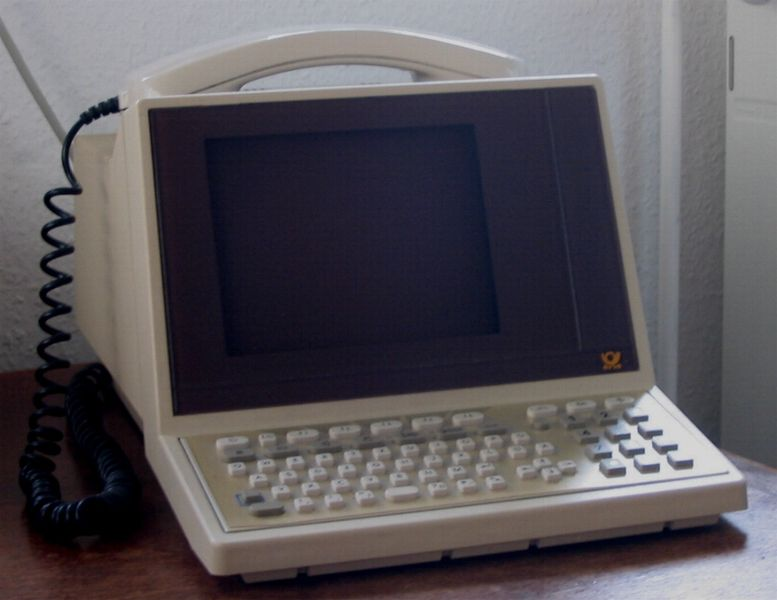
\includegraphics[scale=0.4]{Bilder/777px-Btx_device}
 \caption{Vidphone}
 \label{fig:Vidphone}
\end{figure}

Darin sind ein Fernseher, ein Vidphone und ein einfacher Arbeitscomputer 
mit Drucker integriert.
Per Telekom lassen sich öffentliche Daten abfragen und diverse Dienste (Nachrichten, Verkauf, Telefon- und
Sekretariatsdienste) abonnieren.
Die Interpretation als Datennetz für DFÜ verträgt sich auch mit den Romanen, die oft erfordern, dass der Decker auf das
Konzerngelände gebracht wird, um dort interne Anschlüsse anzuzapfen, statt von außen den durch ICE bestgesicherten
Einwahlknoten (SAN) zu passieren (lässt sich wie ein Firewall- und Loginsystem verstehen).

Die Matrix wird als virtuelle Realität dargestellt, in der alle maschinellen und programmierten Objekte und Vorgänge von
dreidimensionalen, geometrischen Symbolen repräsentiert werden.
Diese Bilder sind nur im Gehirn des Deckers real, das direkt mit diesen Objekten kommunizieren kann, bzw. Teil des 
Computers wird.

In den Regeln werden als Vergleich Computerspiele herangezogen; natürlich damalige Spiele und die waren grafisch sehr
elementar gestaltet, z.B. durch untexturierte, ggf. gefärbte Vektorgrafiken, siehe Abbildung \ref{fig:Matrix2050}.
\begin{figure}[ht]
 \centering
 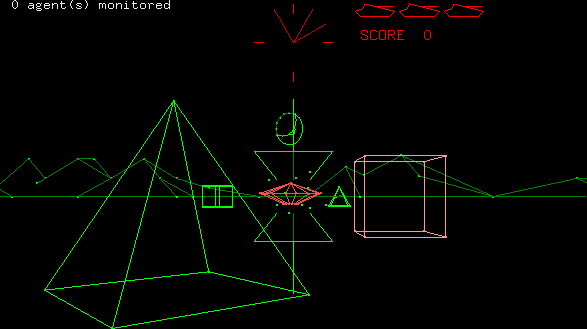
\includegraphics[scale=0.6]{Bilder/battlezone}
 \caption{Blick in die Matrix im Jahre 2050}
 \label{fig:Matrix2050}
\end{figure}

Dies verträgt sich auch mit der Darstellung der Matrix im 2er Grundbuch, wo die Knoten aus einfachen, geometrischen Formen
bestehen.
Erst neuere Cyberdecks, ab \textit{Virtual Realities 2.01D} besitzen einen Realitätsfilter, der die Objekte nach Wunsch 
des Deckers darstellen kann.
Weitere Ausnahmen gibt es auch, wenn der Systemdesigner des Netzes Wert auf optische Spielereien legt (z.B. fliegende
Lederhäute in der Matrix des Modedesigners Jacobi oder die CPU als Burghof bei Renraku in der Deutschlandtrilogie).

Programme, die teure Maßanfertigungen sind, besitzen ebenfalls meist ein eigenes Design, vor allem ICE-Programme 
(Römische Soldaten, Drachen, Wachhunde, \dots) oder Personaprogramme von Deckern.
Im Laufe der Zeit (bspw. 2054) werden komplexere grafische Darstellungen geläufiger, die meisten Systeme sehen aber 
dennoch spartanisch aus.
2060, passend zu den 3er Regeln, gibt es das fest definierte Matrixdesign nicht mehr, die Systeme sind aufwändiger
und freier gestaltbar.

Bildtelefonie, SimSinn und Autoleitsysteme werden ebenfalls durch die Matrix geroutet, diese Systeme lassen sich aber 
wie ein VPN interpretieren, die ein in sich gekapseltes, virtuelles Netz repräsentieren, aus dem man normalerweise nicht
herauskommt und deren Zugänge zur Matrix ebenfalls stark gesichert sind.

Laut \textit{Deutschland in den Schatten} bezeichnet man die Matrix in der ADL auch als ISDN2 oder ISDN pro.
In der beschriebenen Form existiert sie seit 2041 in Deutschland, hat zur Spielzeit der Regeln (also 10-20 Jahre später) 
aber ihre Kapazitätsgrenzen erreicht, so dass man zu Arbeitszeiten Glück haben muss, eine bestehende Verbindung hinzukriegen!

Weil die Datennetze keine Webpräsenzen darstellen und die Konzerne ihre SANs abriegeln, besteht auch kein Bedarf für
Suchmaschinen (dafür begibt man sich ja gerade in einen Knoten und startet da sein Schmökerprogramm)
oder gar Zusatzdienste wie Googlemaps (man kann natürlich in die Matrix des Katasteramtes decken oder sich Papierkarten oder
digitale Karten kaufen) oder soziale Netze.
Denkbar sind Chaträume in illegalen Knoten, die nur von Deckern betrieben und besucht werden.
Das Austauschen von Nachrichten zwischen Personaprogrammen erfordert aber auch keinen speziellen Raum, hauptsache man
findet einen Knoten, in dem man sich zeitgleich aufhält, um in Kontaktreichweite zu gelangen.

Matrixcafés in Form von heutigen Internetcafés es gibt es entsprechend auch nicht, weil man nicht in der Gegend herumsurft
und eher Faxe, Vidphones und Briefpost zur privaten Kommunikation benutzt.
In der Firmenmatrix kann man zusätzlich Telefonkonferenzen schalten, Meldungen zu I/O-Ports schicken, wo sie dann auf
Druckern oder Terminals ausgegeben werden.

Wegen des hohen Aufwands, der exorbitanten Kosten und des prinzipiell geringen Nutzens für Privatleute, kann man
Matrixanschlüsse höchstens ab einem Oberschichtlebensstil als erschwinglich betrachten (und auch nur, wenn der
Kunde wirklich etwas von einem eigenen Anschluss hat); ein legaler Anschluss wird ein paar hundert EC pro Monat kosten, ein
Terminal (Schnecke) ebenfalls (ein Zehntel eines Cyberdecks), ein eigener, simpler Server in Form eines Matrixknotens
vermutlich mindestens 15.000EC bis unendlich; das einfachste Cyberdeck, das ja nur ein Clientsystem ist, kostet bereits fast
7000EC und legale Interfacemodifikationen\footnote{Serverseitig? Oder für Cyberdecks?} kosten nach einem Werbebild im
Deutschlandbuch über 13.000EC, das kauft sich kein normaler Bürger einfach so und die wirklich guten Decks
kosten schon Beträge, für die man ein Auto, eine Wohnung oder gar ein Haus anschafft, worauf der Großteil der Bevölkerung
viele Jahre ansparen muss; nur dass ein Haus nicht jeden Monat veraltet wie ein Cyberdeck nach SOTA\footnote{State of the Art}-Regel.

Für Decking oder sonstige grau-schwarze Aktivitäten von außerhalb eines Konzernnetzes zapft man besser an geeigneter Stelle
die Leitungen an, benötigt dafür aber großes Knowhow, damit die Modifikation dem Netzbetreiber nicht auffällt.
Nutzbare Komverbindungen werden als Jackpoints bezeichnet, von denen es legale und illegale gibt.
Dies können Tridphones, Workstations, Geräteinterfaces oder andere Möglichkeiten sein, sich ins Glasfasernetz zu klinken.

Man darf auch nicht vergessen, dass alle Cyberdecks und Computer in der Matrix Spuren hinterlassen, außer wenn sie von
Deckern modifiziert worden sind, dies nicht mehr zu tun.

Auf Geschwindigkeiten und Kapazitäten von Decks muss nicht eingegangen werden, weil dazu Megapulse und Megapulse pro
Kampfrunde verwendet werden, die es in der Realität eh nicht gibt.
 
\subsection{Cyberware}
Die Regeln für Cyberware beschreiben sie eigentlich ausreichend; sie muss implantiert werden und mit den Nervenbahnen
verbunden werden, anders als Metallschrauben, Zahnfüllungen und Herzschrittmacher, die nicht mit dem Gehirn kommunizieren
müssen.
Es handelt sich also um nichtnatürliche Implantate, die über spezielle Interfaces an das Gehirn gekoppelt sind, welches 
diese Teile als Fremdkörper identifiziert.
Laut \textit{Mensch und Maschine 3.01D} sind die dadurch auftretenden Probleme des Gehirns die Ursache des Essenzverlustes.
Essenz wird in \textit{Shadowrun 2.01D} als Solidität des zentralen Nervensystems und des Geistes beschrieben,
mit einer Essenz unter 0 stirbt man wenig später und auch mit niedriger, positiver Essenz wird man melancholisch und
verzweifelt.
Leute mit niedriger Essenz wandeln am Rande des Wahnsinns.

Das impliziert übrigens, da ein schwerer oder tödlicher Schaden einen Essenzverlust bedeuten kann, dass ein Straßensamurai
durch eine Verwundung, Drogenabhängigkeit, Traumata und chirurgische Eingriffe trotzdem durch den Essenzverlust stirbt,
obwohl jeder andere es überstanden hätte!

Die Natur der Komponenten macht es schwierig, sie vollständig im Körper zu integrieren. Wie gut sie auch getarnt sein mögen,
Cyberware-Teile sehen laut \textit{Shadowtech} immer etwas deplaziert aus (zu glatte Bewegungen, zu schnelle Reaktionen, zu
perfektes Erscheinungsbild usw.).
Nach \textit{Mensch und Maschine} ist die grundlegende Tarnstufe $8$, für Alpha-, Beta-, Deltaware um je $+2$ größer.
Je nach Zusatzoptionen der Geräte und je Länge der Beobachtungsdauer lässt sich Cyberware auch immer leichter erkennen.
Ein Charakter mit einer Essenz zwischen 0-3 besitzt laut \textit{Mensch und Maschine} eine um eins kleinere Tarnstufe.

Man sollte aber darauf achten, den Regeln für Cyberware und soziale Interaktion besondere Betonung zu verleihen, weil die
Ganzheit des Körpers wichtig und die Nutzung von Cyberware als Form von Selbstverstümmelung eher abstoßend wirkt.
Hinzu kommt, dass viele Cyberwareimplantate illegal sind, was den Leuten auch prinzipiell bekannt sein dürfte, wenn auch
nicht im Detail, schließlich ist nicht jeder Anwalt.
Implantierte Waffen können aber auch von Laien als illegal erkannt werden und Reflexbooster ebenfalls, weil das ein 
Implantat ist, das in jeder Straßensamurai- oder Urban Brawl-Tridshow als Implantat für Kriminelle oder Sicherheitskräfte
dargestellt wird und offensichtlich nicht im Supermarkt herumliegt.
\end{document}